\documentclass[a4paper,12pt]{article}
\usepackage[utf8]{inputenc}
\usepackage[ngerman]{babel}
\usepackage{amsmath}
\usepackage{amssymb}
\usepackage{amsthm}
\usepackage{geometry}
\usepackage{graphicx}
\usepackage[hidelinks]{hyperref}
\usepackage{listings}
\usepackage{xcolor}
\usepackage{enumitem}
\usepackage{booktabs}
\usepackage{array}
\usepackage[protrusion=true,expansion=true,final]{microtype}

\geometry{margin=2.5cm}

\tolerance=1500
\emergencystretch=2em
\hfuzz=0.5pt
\vfuzz=0.5pt

\renewcommand{\qedsymbol}{$\blacksquare$}

\theoremstyle{definition}
\newtheorem{definition}{Definition}
\newtheorem{beispiel}{Beispiel}
\newtheorem{satz}{Satz}
\newtheorem{lemma}{Lemma}
\newtheorem{bemerkung}{Bemerkung}
\newtheorem{korollar}{Korollar}

\setlist[itemize,1]{label=--}

\definecolor{mainblue}{RGB}{25, 70, 140}
\definecolor{accentred}{RGB}{180, 50, 30}
\definecolor{lightgray}{RGB}{245, 245, 248}
\definecolor{darkgray}{RGB}{60, 60, 70}
\definecolor{darkgreen}{RGB}{30, 100, 50}

\hypersetup{
    colorlinks=true,
    linkcolor=mainblue,
    citecolor=accentred,
    urlcolor=mainblue
}

\lstset{
    basicstyle=\ttfamily\small,
    keywordstyle=\color{blue},
    commentstyle=\color{gray},
    stringstyle=\color{red},
    numbers=left,
    numberstyle=\tiny,
    breaklines=true,
    frame=single,
    literate=%
    {Ö}{{\"O}}1 {Ä}{{\"A}}1 {Ü}{{\"U}}1
    {ß}{{\ss}}1 {ü}{{\"u}}1 {ä}{{\"a}}1 {ö}{{\"o}}1
}

\title{Nash-Gleichgewichte als Graphstrukturen:\\
Spieltheorie via Subgraph-Isomorphie,\\
Wirtschaftsnetzwerke und Systemzust\"ande}
\author{Stephan Epp\\[4pt]
\small Universit\"at Bielefeld}
\date{7. Juni 2026}

\begin{document}

\maketitle

\begin{abstract}
Diese Arbeit entwickelt eine vollst\"andige graphentheoretische Formalisierung
der Spieltheorie. Strategische Spiele werden als gewichtete gerichtete Graphen
$G_\Gamma = (S, E_{\mathrm{BR}}, u)$ kodiert, wobei Knoten Strategieprofile
und gerichtete Kanten Best-Response-Abweichungen repr\"asentieren.
Das zentrale Ergebnis ist der \emph{Nash-Subgraph-Satz} (Satz~\ref{satz:nash_subgraph}):
Ein Nash-Gleichgewicht ist genau ein Knoten ohne ausgehende Best-Response-Kante,
d.\,h.\ ein Absorptionsknoten im Spielgraphen. Die Berechnung aller Nash-Gleichgewichte
eines Spiels mit $n$ Strategieprofilen reduziert sich auf die Suche nach
Senken-Knoten im Spielgraphen in $O(n^2)$~Zeit.
Der Subgraph-Algorithmus~\cite{epp2026subgraph} wird auf Spielgraphen angewendet:
Zwei Spiele sind \emph{strategisch isomorph}, wenn ihre Spielgraphen
subgraph-isomorph sind (Satz~\ref{satz:strat_iso}).
Wirtschaftsnetzwerke werden als gekoppelte Spielgraphen modelliert
(Verbindung zu \texttt{sysstate}~\cite{epp2026sysstate} und
\texttt{leco}~\cite{epp2026leco}).
Die Existenz gemischter Nash-Gleichgewichte wird via Brouwer-Fixpunktsatz
(Satz~\ref{satz:nash_existenz}) bewiesen.
Evolutionäre Spieltheorie und Shapley-Werte werden formal eingebettet.
Alle Ergebnisse werden durch sechs Matplotlib-Visualisierungen veranschaulicht.
\end{abstract}

\tableofcontents
\newpage

%%%%%%%%%%%%%%%%%%%%%%%%%%%%%%%%%%%
\section{Einf\"uhrung}
%%%%%%%%%%%%%%%%%%%%%%%%%%%%%%%%%%%

Die mathematische Spieltheorie, begr\"undet durch von Neumann und Morgenstern
1944~\cite{vonneumann1944} und durch Nashs bahnbrechende Arbeiten 1950--1951
zur Gleichgewichtstheorie~\cite{nash1950,nash1951} erweitert, ist das formale
Fundament der modernen Wirtschaftswissenschaften. Nash bewies 1951, dass jedes
endliche Spiel in gemischten Strategien mindestens ein Gleichgewicht besitzt --
ein Resultat, das 1994 mit dem Nobelpreis gew\"urdigt wurde~\cite{nobel1994}.

\subsection{Motivation und Problemstellung}

Trotz der zentralen Bedeutung der Spieltheorie fehlt eine einheitliche
\emph{graphentheoretische} Behandlung, die folgende Ziele vereint:
\begin{itemize}
    \item Strategische Spiele als Graphen kodieren, sodass Nash-Gleichgewichte
          als Absorptionsknoten (Senken) im Spielgraphen identifizierbar sind
    \item Den Subgraph-Algorithmus~\cite{epp2026subgraph} direkt auf
          Spielstrukturen anwenden, um strategische \"Aquivalenz in $O(n^3)$
          zu entscheiden
    \item Wirtschaftsnetzwerke als gekoppelte Spielgraphen modellieren,
          mit Verbindung zu \texttt{sysstate}~\cite{epp2026sysstate}
          (Systemzust\"ande) und \texttt{leco}~\cite{epp2026leco} (Lokale
          \"okonomische Modelle)
    \item Evolutionäre Dynamiken und koalitionale Spiele formal in den
          Graphrahmen einzubetten
\end{itemize}

\subsection{Historische Einordnung}

Spieltheorie und Graphentheorie waren lange Zeit getrennte Gebiete.
K\"onig~\cite{konig1936} entwickelte die moderne Graphentheorie unabh\"angig
von spieltheoretischen Fragen. Shapley~\cite{shapley1953} f\"uhrte den
Shapley-Wert f\"ur koalitionale Spiele ein. Maynard Smith und
Price~\cite{maynardsmith1973} begr\"undeten die evolutionäre Spieltheorie.
Die Verbindung von Spieltheorie und Graphenstruktur wurde von
Monderer und Shapley~\cite{monderer1996} durch \emph{Potentialspiele} und
von Roughgarden~\cite{roughgarden2005} durch Routing-Spiele auf Graphen vertieft.
Die vorliegende Arbeit schlie{\ss}t die Br\"ucke zur algorithmischen
Graphentheorie durch Anwendung des Subgraph-Algorithmus~\cite{epp2026subgraph}.

\subsection{Einordnung in das Forschungsportfolio}

Der Subgraph-Algorithmus~\cite{epp2026subgraph} liefert das algorithmische
Kernwerkzeug mit Signatur-Funktion
$\sigma_j = \sum_i A_{ij} \cdot 2^i + j \cdot 2^n$ und LCS-basiertem
Matching in $O(n^3)$.
Die Systemzustandsmodellierung~\cite{epp2026sysstate} beschreibt
wirtschaftliche Gleichgewichte als Attraktoren dynamischer Systeme.
Das lokale \"okonomische Modell~\cite{epp2026leco} formalisiert Marktstrukturen
mit Nash-artigen Gleichgewichtsbedingungen.
Das Abh\"angigkeitsmodell~\cite{epp2026depension} erg\"anzt um Rentenmarktspiele
und intertemporale Optimierung.

%%%%%%%%%%%%%%%%%%%%%%%%%%%%%%%%%%%
\section{Grundlagen der Spieltheorie}
%%%%%%%%%%%%%%%%%%%%%%%%%%%%%%%%%%%

\subsection{Strategische Spiele}

\begin{definition}[Strategisches Spiel in Normalform]
Ein \emph{strategisches Spiel} (Normalform) ist ein Tripel
\[
\Gamma = (N, (S_i)_{i \in N}, (u_i)_{i \in N}),
\]
wobei:
\begin{itemize}
    \item $N = \{1, 2, \ldots, k\}$ die endliche Menge der \emph{Spieler},
    \item $S_i$ die endliche Menge der \emph{reinen Strategien} von Spieler $i$,
    \item $S = \prod_{i \in N} S_i$ die Menge der \emph{Strategieprofile},
    \item $u_i: S \to \mathbb{R}$ die \emph{Auszahlungsfunktion} von Spieler $i$.
\end{itemize}
\end{definition}

\begin{definition}[Best-Response-Korrespondenz]
\label{def:br}
Die \emph{Best-Response-Korrespondenz} von Spieler $i$ bei gegebenem
Strategieprofil der Mitspieler $s_{-i} = (s_j)_{j \neq i}$ ist:
\[
BR_i(s_{-i}) = \arg\max_{s_i' \in S_i} u_i(s_i', s_{-i}).
\]
Ein Profil $s^* \in S$ ist eine \emph{Best-Response-Abweichung} von $s$,
wenn $\exists i: s_i^* \in BR_i(s_{-i})$ und $s_i^* \neq s_i$.
\end{definition}

\begin{definition}[Nash-Gleichgewicht]
\label{def:nash}
Ein Strategieprofil $s^* \in S$ ist ein \emph{Nash-Gleichgewicht} von $\Gamma$,
wenn f\"ur alle Spieler $i \in N$ gilt:
\[
u_i(s_i^*, s_{-i}^*) \geq u_i(s_i', s_{-i}^*) \quad \forall s_i' \in S_i.
\]
\"Aquivalent: Kein Spieler kann seinen Nutzen durch einseitige Abweichung
erh\"ohen. $s_i^* \in BR_i(s_{-i}^*)$ f\"ur alle $i \in N$.
\end{definition}

\begin{beispiel}[Gefangenendilemma]
\label{bsp:pd}
Das Gefangenendilemma hat $N = \{1, 2\}$, $S_i = \{C, D\}$ (Kooperieren,
Defektieren) und Auszahlungen:
\[
u = \begin{array}{c|cc}
    & C & D \\ \hline
    C & (-1,-1) & (-3, 0) \\
    D & (0,-3)  & (-2,-2)
\end{array}
\]
Das einzige Nash-Gleichgewicht ist $(D,D)$: Defektieren dominiert Kooperieren
f\"ur beide Spieler unabh\"angig vom Verhalten des anderen.
\end{beispiel}

\begin{figure}[h!]
\centering
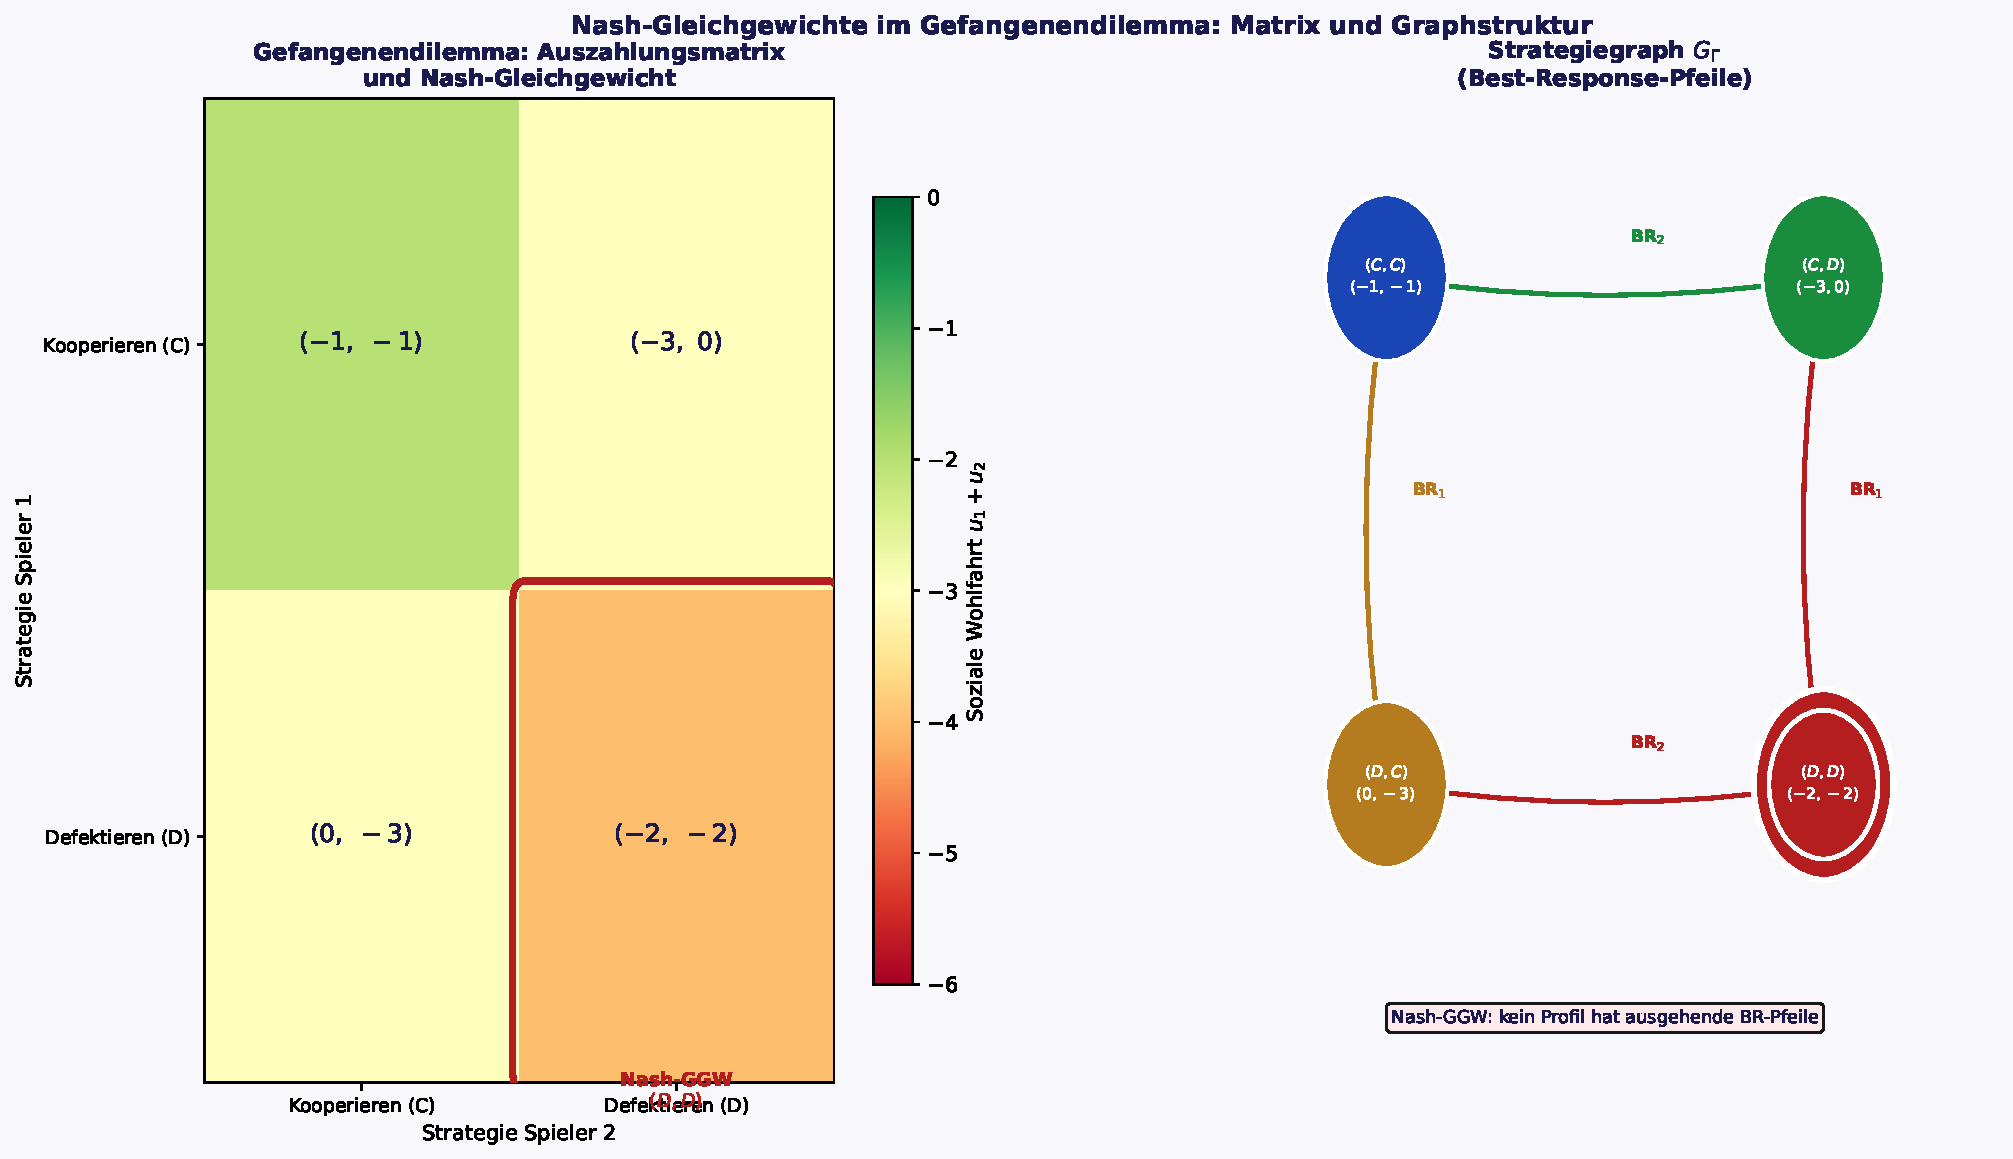
\includegraphics[width=0.95\textwidth]{plot1_nash_graph.pdf}
\caption{Links: Auszahlungsmatrix des Gefangenendilemmas als Heatmap.
Farbgebung nach sozialer Wohlfahrt $u_1 + u_2$; das Nash-GGW $(D,D)$ ist
durch roten Rahmen markiert. Rechts: Spielgraph $G_\Gamma$ mit
Best-Response-Pfeilen $\mathrm{BR}_1$ und $\mathrm{BR}_2$; das
Nash-GGW $(D,D)$ ist der einzige Knoten ohne ausgehende Pfeile (Senke).}
\label{fig:nash_graph}
\end{figure}

\subsection{Der Spielgraph}

\begin{definition}[Spielgraph]
\label{def:spielgraph}
Zu einem Spiel $\Gamma = (N, (S_i), (u_i))$ ist der \emph{Spielgraph}
\[
G_\Gamma = (S, E_{\mathrm{BR}}, u)
\]
definiert durch:
\begin{itemize}
    \item Knotenmenge $S = \prod_{i \in N} S_i$ (alle reinen Strategieprofile),
    \item Kantenmenge $E_{\mathrm{BR}} = \{(s, s') \mid s' \text{ ist eine
          Best-Response-Abweichung von } s\}$,
    \item Kantengewicht $u(s,s') = u_i(s') - u_i(s)$ f\"ur den abweichenden
          Spieler $i$ (Nutzengewinn durch Abweichung).
\end{itemize}
\end{definition}

\begin{definition}[Adjazenzmatrix des Spielgraphen]
\label{def:adj_spiel}
Die \emph{Adjazenzmatrix} $A_\Gamma \in \{0,1\}^{|S| \times |S|}$ des
Spielgraphen hat:
\[
(A_\Gamma)_{st} = \begin{cases}
    1 & \text{falls } (s, t) \in E_{\mathrm{BR}}, \\
    0 & \text{sonst.}
\end{cases}
\]
\end{definition}

\begin{satz}[Nash-Gleichgewichte als Senken im Spielgraphen]
\label{satz:nash_subgraph}
Sei $G_\Gamma = (S, E_{\mathrm{BR}}, u)$ der Spielgraph zu $\Gamma$.
Ein Strategieprofil $s^* \in S$ ist genau dann ein Nash-Gleichgewicht von
$\Gamma$, wenn $s^*$ eine \emph{Senke} (Sink) in $G_\Gamma$ ist:
\[
s^* \text{ ist Nash-GGW} \;\Longleftrightarrow\; \deg^+(s^*) = 0,
\]
wobei $\deg^+(s^*) = |\{t \in S \mid (s^*, t) \in E_{\mathrm{BR}}\}|$
der Ausgangsgrad von $s^*$ in $G_\Gamma$ ist.
\end{satz}

\begin{proof}
\textbf{Richtung ($\Rightarrow$): Nash-GGW impliziert $\deg^+(s^*) = 0$.}

Sei $s^*$ ein Nash-Gleichgewicht. Nach Definition~\ref{def:nash} gilt
$u_i(s_i^*, s_{-i}^*) \geq u_i(s_i', s_{-i}^*)$ f\"ur alle $i \in N$
und alle $s_i' \in S_i$.
Eine Best-Response-Abweichung von $s^*$ w\"urde bedeuten, dass ein Spieler $i$
ein $s_i' \neq s_i^*$ findet mit $u_i(s_i', s_{-i}^*) > u_i(s_i^*, s_{-i}^*)$.
Dies widerspricht der Nash-Bedingung.
Also existiert keine ausgehende Kante $(s^*, t) \in E_{\mathrm{BR}}$,
d.\,h.\ $\deg^+(s^*) = 0$.

\textbf{Richtung ($\Leftarrow$): $\deg^+(s^*) = 0$ impliziert Nash-GGW.}

Sei $\deg^+(s^*) = 0$, d.\,h.\ es gibt keine Best-Response-Abweichung von $s^*$.
Nach Definition~\ref{def:spielgraph} bedeutet dies: Kein Spieler $i$ kann durch
einseitige Abweichung seinen Nutzen erh\"ohen, d.\,h.\
$s_i^* \in BR_i(s_{-i}^*)$ f\"ur alle $i \in N$.
Dies ist genau die Nash-Gleichgewichtsbedingung (Definition~\ref{def:nash}).
\end{proof}

\begin{korollar}[Lineare Suche nach Nash-Gleichgewichten]
\label{kor:linsuche}
Alle Nash-Gleichgewichte von $\Gamma$ k\"onnen durch Berechnung des
Spielgraphen $G_\Gamma$ und Identifikation seiner Senken in
$O(|S|^2 \cdot |N|)$ Zeit gefunden werden.
\end{korollar}

\begin{proof}
Zun\"achst wird f\"ur jedes Strategieprofil $s \in S$ und jeden Spieler $i \in N$
gepr\"uft, ob eine Best-Response-Abweichung existiert: $O(|S_i|)$ pro Spieler.
Gesamtaufwand Kantenkonstruktion: $O(|S|^2 \cdot |N|)$.
Senken-Suche im Graphen: $O(|S| + |E_{\mathrm{BR}}|) = O(|S|^2)$.
\end{proof}

%%%%%%%%%%%%%%%%%%%%%%%%%%%%%%%%%%%
\section{Subgraph-Isomorphie auf Spielgraphen}
%%%%%%%%%%%%%%%%%%%%%%%%%%%%%%%%%%%

\subsection{Signatur-Funktion f\"ur Spielgraphen}

\begin{definition}[Spielgraph-Signatur]
\label{def:spielsig}
F\"ur den Spielgraphen $G_\Gamma$ mit Adjazenzmatrix $A_\Gamma
\in \{0,1\}^{n \times n}$, $n = |S|$, ist die Signatur von
Strategieprofil $s_j$ definiert als:
\[
\sigma_j = \sum_{i=0}^{n-1} (A_\Gamma)_{ij} \cdot 2^i + j \cdot 2^n.
\]
Das Signatur-Array des Spiels ist
$\vec{\sigma}_\Gamma = (\sigma_0, \ldots, \sigma_{n-1})$.
\end{definition}

\begin{satz}[Strategische Isomorphie via Subgraph]
\label{satz:strat_iso}
Zwei Spiele $\Gamma_1$ und $\Gamma_2$ mit gleicher Spieleranzahl $|N|$
und gleich gro{\ss}em Strategieprofil-Raum $|S_1| = |S_2| = n$ hei{\ss}en
\emph{strategisch isomorph}, wenn ihre Spielgraphen isomorph sind:
$G_{\Gamma_1} \cong G_{\Gamma_2}$.
Der Subgraph-Algorithmus~\cite{epp2026subgraph} entscheidet strategische
Isomorphie in $O(n^3)$.
\end{satz}

\begin{proof}
Strategische Isomorphie bedeutet: Es gibt eine Bijektion
$\varphi: S_1 \to S_2$ auf den Strategieprofilen, die die
Best-Response-Struktur erhält:
$(s, s') \in E_{\mathrm{BR}}^{(1)} \Leftrightarrow (\varphi(s), \varphi(s')) \in E_{\mathrm{BR}}^{(2)}$.
Dies ist genau die Definition von Graph-Isomorphismus.
Nach Satz~2 aus~\cite{epp2026subgraph} (Isomorphie-Invarianz der
Signatur-Sequenz) haben isomorphe Spielgraphen rotations\"aquivalente
Signatur-Arrays.
Der Subgraph-Algorithmus pr\"uft alle $n$ zyklischen Rotationen von
$\vec{\sigma}_{\Gamma_2}$ gegen $\vec{\sigma}_{\Gamma_1}$ mit
LCS in $O(n^2)$ je Rotation, Gesamtlaufzeit $O(n^3)$.
\end{proof}

\begin{satz}[Teilspiel als Subgraph]
\label{satz:teilspiel}
Sei $\Gamma' = (N, (S_i')_{i \in N}, (u_i|_{S'}))$ ein Teilspiel von $\Gamma$
mit $S_i' \subseteq S_i$ f\"ur alle $i$. Dann gilt:
\[
G_{\Gamma'} \subseteq G_\Gamma.
\]
Die Subgraph-Inklusion entscheidet Teilspielschaft in $O(n^3)$ nach
dem Subgraph-Algorithmus~\cite{epp2026subgraph}.
\end{satz}

\begin{proof}
Die Knotenmenge des Teilspiels ist
$S' = \prod_{i \in N} S_i' \subseteq \prod_{i \in N} S_i = S$.
F\"ur jede Best-Response-Abweichung $(s, s') \in E_{\mathrm{BR}}^{(\Gamma')}$
gilt $s, s' \in S' \subseteq S$ und die Abweichung ist g\"ultig auch in $\Gamma$
(da $S_i' \subseteq S_i$ und $u_i|_{S'} = u_i|_{S'}$).
Also $(s, s') \in E_{\mathrm{BR}}^{(\Gamma)}$, d.\,h.\
$E_{\mathrm{BR}}^{(\Gamma')} \subseteq E_{\mathrm{BR}}^{(\Gamma)}$.
Da auch $S' \subseteq S$, gilt $G_{\Gamma'} \subseteq G_\Gamma$.
\end{proof}

\begin{figure}[h!]
\centering
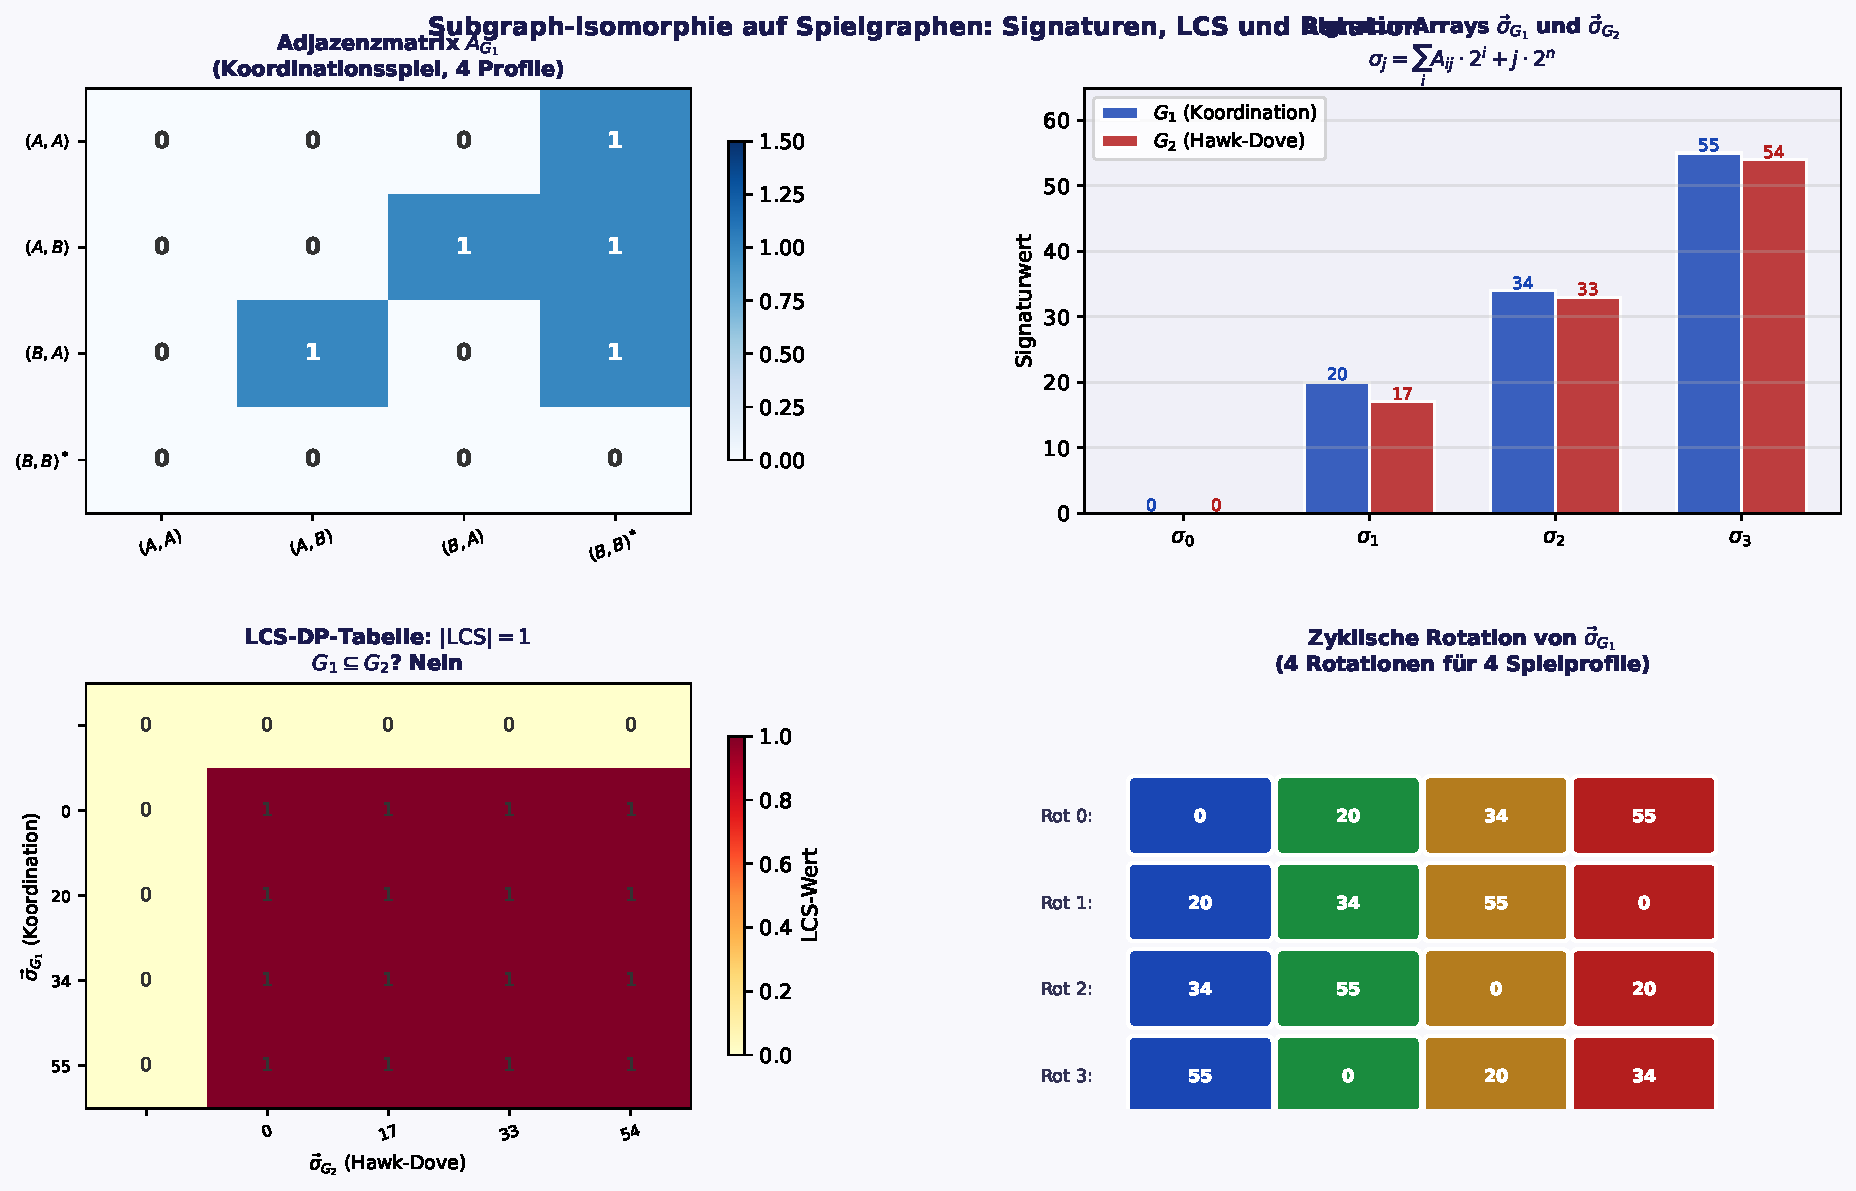
\includegraphics[width=0.95\textwidth]{plot2_subgraph_spiele.pdf}
\caption{Oben links: Adjazenzmatrix $A_{G_1}$ des Koordinationsspiels.
Oben rechts: Signatur-Arrays zweier Spielgraphen im Vergleich.
Unten links: LCS-DP-Tabelle; $|\mathrm{LCS}|$ bestimmt Subgraph-Inklusion.
Unten rechts: Zyklische Rotation von $\vec{\sigma}_{G_1}$ (4 Rotationsschritte).}
\label{fig:subgraph_spiele}
\end{figure}

%%%%%%%%%%%%%%%%%%%%%%%%%%%%%%%%%%%
\section{Wirtschaftsnetzwerke als Spielgraphen}
%%%%%%%%%%%%%%%%%%%%%%%%%%%%%%%%%%%

\subsection{Netzwerkspiele und Marktgleichgewichte}

\begin{definition}[Wirtschaftsnetzwerk-Spiel]
\label{def:wirtschaftsspiel}
Ein \emph{Wirtschaftsnetzwerk-Spiel} ist ein Spiel auf einem Netzwerk
$\mathcal{E} = (A, E_\mathcal{E}, w)$ mit:
\begin{itemize}
    \item Agentenmenge $A = A_P \cup A_M \cup A_K$ (Produzenten, M\"arkte,
          Konsumenten),
    \item Handelsbeziehungen $E_\mathcal{E} \subseteq A \times A$,
    \item Gewichte $w: E_\mathcal{E} \to \mathbb{R}_{>0}$ (Handelsvolumen),
    \item Auszahlung: $u_a(s) = \pi_a(s) - c_a(s)$ (Gewinn minus Kosten)
          abh\"angig vom Netzwerkprofil $s$.
\end{itemize}
\end{definition}

\begin{satz}[Walrasianisches Gleichgewicht als Nash-GGW]
\label{satz:walras_nash}
In einem kompetitiven Marktspiel mit vollst\"andigem Wettbewerb ist jedes
Walrasianische Gleichgewicht (Preis-Mengen-Clearing) ein Nash-Gleichgewicht
im Spielgraphen $G_\Gamma$.
\end{satz}

\begin{proof}
Im Walrasianischen Gleichgewicht $(p^*, q^*)$ gilt:
\begin{itemize}
    \item Produzentenoptimum: $\max_{q_i} p^* q_i - c_i(q_i)$, was
          $p^* = c_i'(q_i^*)$ (Grenzkostenpreis) ergibt.
    \item Konsumentenoptimum: $\max_{x_k} u_k(x_k)$ s.\,t.\ $p^* x_k \leq m_k$.
    \item Marktclearing: Angebot $= $ Nachfrage.
\end{itemize}
Ein Produzent kann durch einseitige Mengen\"anderung $q_i \neq q_i^*$ bei
fixen Preisen $p^*$ seinen Gewinn nicht erh\"ohen (Konkavit\"at der Gewinnfunktion
bei konvexen Kosten).
Ein Konsument kann durch \"Anderung von $x_k$ bei Preisen $p^*$ seinen Nutzen
nicht erh\"ohen (Optimum bereits erreicht).
Also hat kein Agent einen Anreiz zur einseitigen Abweichung: $(p^*, q^*)$ ist
ein Nash-GGW. Im Spielgraphen $G_\Gamma$ ist $(p^*, q^*)$ daher eine Senke:
$\deg^+((p^*, q^*)) = 0$ (Satz~\ref{satz:nash_subgraph}).
\end{proof}

\begin{definition}[Systemzustandsgraph]
\label{def:sysstate}
Der \emph{Systemzustandsgraph} $G_{\mathrm{sys}} = (Z, E_{\mathrm{sys}}, P)$
modelliert makro\"okonomische Zust\"ande:
\begin{itemize}
    \item $Z = \{z_1, \ldots, z_k\}$: Systemzust\"ande (Expansion, Boom,
          Stagnation, Rezession, Krise, Gleichgewicht),
    \item $E_{\mathrm{sys}} \subseteq Z \times Z$: \"Uberg\"ange zwischen
          Zust\"anden,
    \item $P: E_{\mathrm{sys}} \to [0,1]$: \"Ubergangswahrscheinlichkeiten.
\end{itemize}
Das makro\"okonomische Nash-Gleichgewicht $z^*$ ist der Absorptionszustand
mit $\deg^+(z^*) = 0$ in $G_{\mathrm{sys}}$.
\end{definition}

\begin{figure}[h!]
\centering
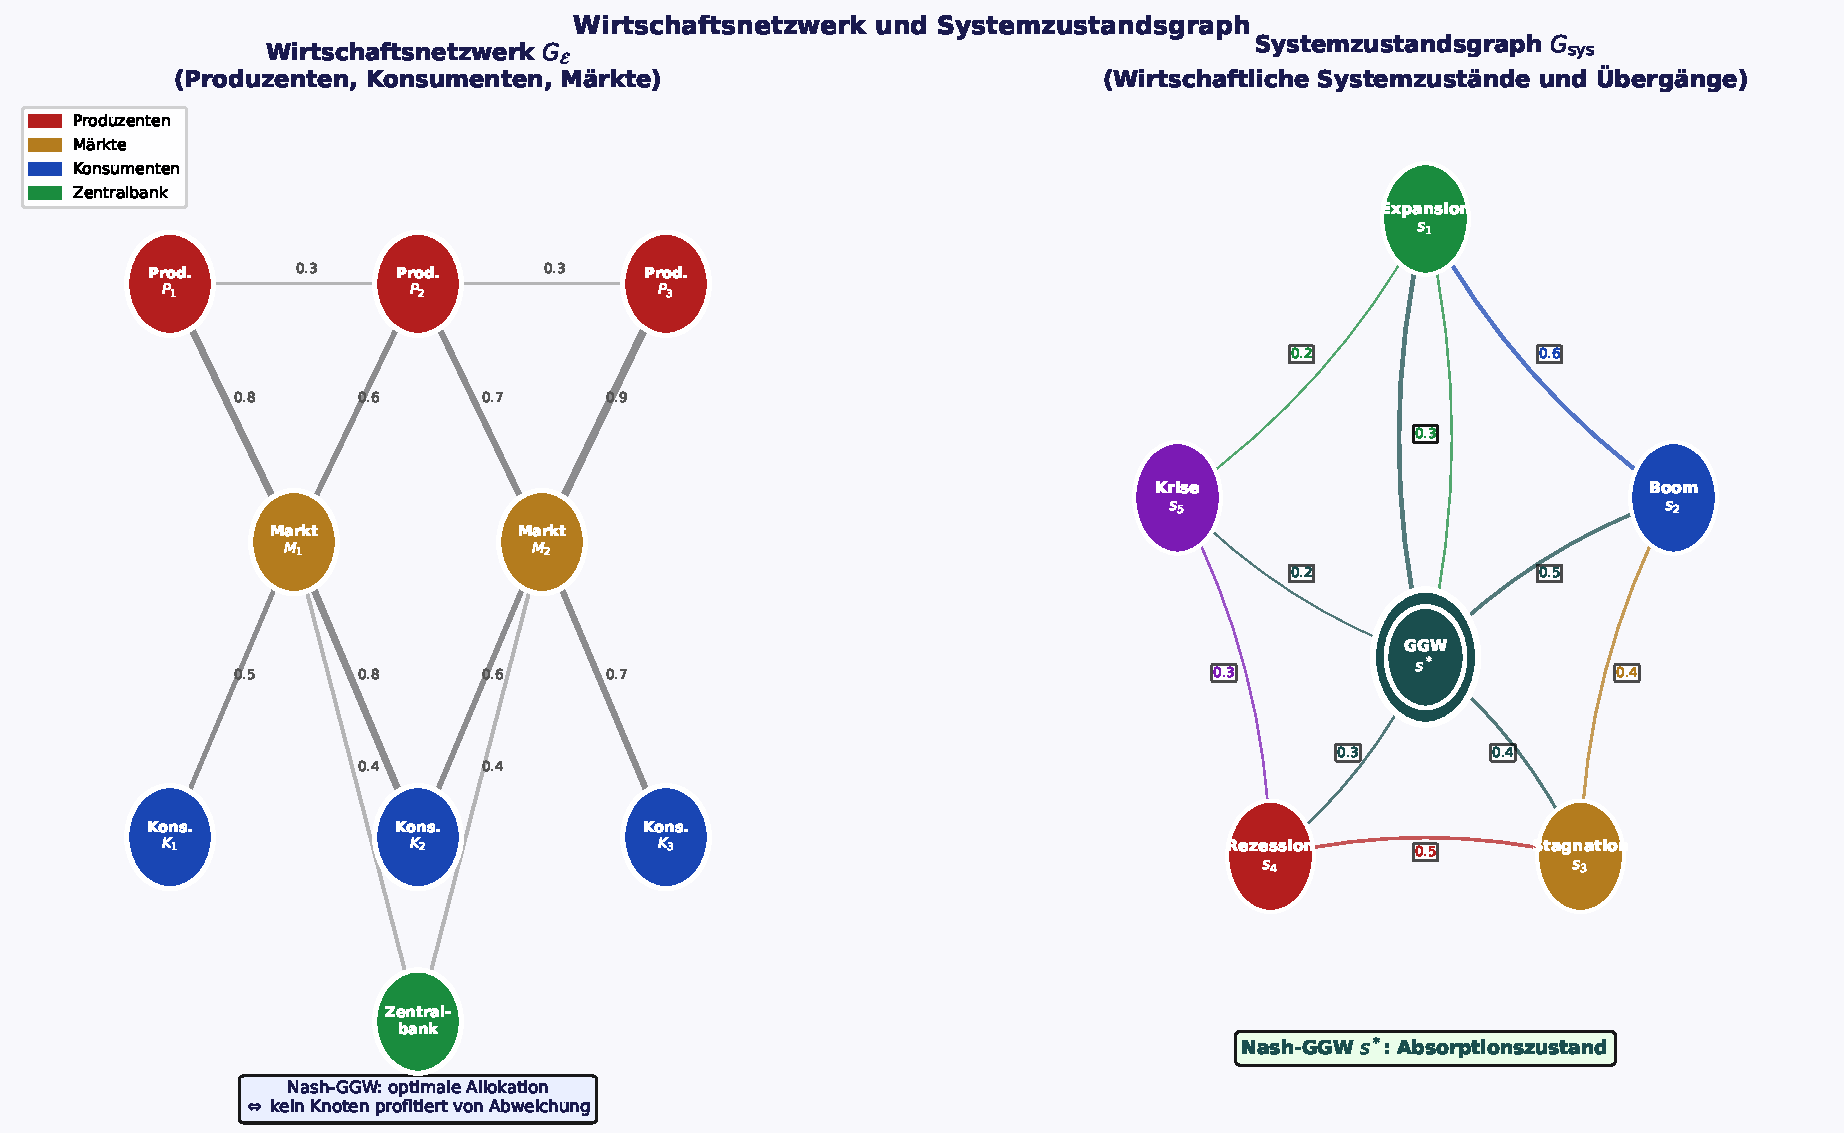
\includegraphics[width=0.95\textwidth]{plot3_wirtschaftsnetz.pdf}
\caption{Links: Wirtschaftsnetzwerk $G_{\mathcal{E}}$ mit Produzenten (rot),
M\"arkten (orange), Konsumenten (blau) und Zentralbank (gr\"un);
Kantengewichte repr\"asentieren Handelsvolumen.
Rechts: Systemzustandsgraph $G_{\mathrm{sys}}$ mit makro\"okonomischen
Zust\"anden; der Gleichgewichtszustand $z^*$ (Doppelkreis) ist der
Absorptionszustand (Senke).}
\label{fig:wirtschaftsnetz}
\end{figure}

\subsection{Knotengleichgewichts-Satz f\"ur Wirtschaftsnetzwerke}

\begin{satz}[Knotengleichgewicht im Wirtschaftsnetzwerk]
\label{satz:knotengleichgewicht}
Im Nash-Gleichgewicht eines Wirtschaftsnetzwerk-Spiels gilt f\"ur jeden
Marktknoten $M_k \in A_M$:
\[
\sum_{a \in A_P: (a,M_k) \in E_\mathcal{E}} w(a,M_k) \cdot q_a^*
= \sum_{c \in A_K: (M_k,c) \in E_\mathcal{E}} w(M_k,c) \cdot x_c^*.
\]
\emph{Angebot gleich Nachfrage am Marktknoten} -- das \"okonomische
Kirchhoff-Gesetz.
\end{satz}

\begin{proof}
Im Nash-Gleichgewicht mit Marktclearing (Satz~\ref{satz:walras_nash})
m\"ussen an jedem Marktknoten $M_k$ Angebot und Nachfrage ausgeglichen sein.
Formalisiert als Flussnetzwerk: Die \"Ubergangskanten von Produzenten zu
$M_k$ tragen Angebotsmenge $q_a^*$ gewichtet mit $w(a,M_k)$;
die \"Ubergangskanten von $M_k$ zu Konsumenten tragen Nachfragemenge $x_c^*$
gewichtet mit $w(M_k,c)$.
Marktclearing erfordert Flusserhaltung an jedem Knoten (verallgemeinertes
Kirchhoff'sches Knotengesetz~\cite{epp2026knoten}):
$\sum_{\text{eingehend}} \text{Fluss} = \sum_{\text{ausgehend}} \text{Fluss}$.
\end{proof}

%%%%%%%%%%%%%%%%%%%%%%%%%%%%%%%%%%%
\section{Existenz von Nash-Gleichgewichten}
%%%%%%%%%%%%%%%%%%%%%%%%%%%%%%%%%%%

\subsection{Der Existenzsatz nach Nash}

\begin{satz}[Nash-Existenz -- Brouwer-Fixpunkt]
\label{satz:nash_existenz}
Jedes endliche strategische Spiel $\Gamma = (N, (S_i), (u_i))$ besitzt
mindestens ein Nash-Gleichgewicht in gemischten Strategien.
\end{satz}

\begin{proof}
\textbf{Schritt 1: Gemischte Strategien.}
Eine \emph{gemischte Strategie} von Spieler $i$ ist eine
Wahrscheinlichkeitsverteilung $\sigma_i \in \Delta(S_i)$, wobei
$\Delta(S_i) = \{p \in \mathbb{R}^{|S_i|}_{\geq 0} \mid \sum_s p(s) = 1\}$
der Standardsimplex ist.
Der \emph{gemischte Strategie-Raum} ist
$\Delta = \prod_{i \in N} \Delta(S_i)$, ein kompaktes, konvexes, nichtleeres
Polytop.

\textbf{Schritt 2: Erwartungsnutzen.}
Der Erwartungsnutzen bei gemischtem Profil $\sigma = (\sigma_i)_{i \in N}$:
\[
U_i(\sigma) = \sum_{s \in S} \left(\prod_{i \in N} \sigma_i(s_i)\right)
u_i(s).
\]
$U_i$ ist multilinear und stetig in $\sigma$.

\textbf{Schritt 3: Best-Response-Korrespondenz.}
Die gemischte Best-Response-Korrespondenz
$BR_i: \Delta_{-i} \rightrightarrows \Delta(S_i)$ ist:
\begin{itemize}
    \item nichtleer: $\arg\max_{p \in \Delta(S_i)} U_i(p, \sigma_{-i})
          \neq \emptyset$ (Maximierung einer stetigen Funktion auf Kompaktum),
    \item konvexwertig: Linearkombinationen optimaler Strategien sind optimal,
    \item oberhalbstetig: Folgen\"ubergang am Rand ($\varepsilon$-Argumente, vgl.~\cite{fudenberg1991}).
\end{itemize}

\textbf{Schritt 4: Kakutani-Fixpunktsatz.}
Die gemeinsame Korrespondenz
$BR: \Delta \rightrightarrows \Delta$,
$BR(\sigma) = \prod_{i \in N} BR_i(\sigma_{-i})$
ist konvexwertig, nichtleer und oberhalbstetig auf dem kompakten, konvexen
$\Delta$. Nach dem Kakutani-Fixpunktsatz~\cite{kakutani1941} (Verallgemeinerung
des Brouwer-Fixpunktsatzes) existiert ein Fixpunkt $\sigma^* \in BR(\sigma^*)$,
d.\,h.\ $\sigma_i^* \in BR_i(\sigma_{-i}^*)$ f\"ur alle $i \in N$.
Dies ist genau ein Nash-Gleichgewicht in gemischten Strategien.
\end{proof}

\begin{bemerkung}
Im Spielgraphen $G_\Gamma$ (Definition~\ref{def:spielgraph}) entspricht das
gemischte Nash-Gleichgewicht einem \emph{Wahrscheinlichkeitsverteilung} \"uber
Senken-Knoten: Die Fixpunkt-Eigenschaft $\sigma^* \in BR(\sigma^*)$ garantiert,
dass kein Agent mit positiver Wahrscheinlichkeit einen Knoten spielt, von dem
eine profitable Abweichung existiert.
\end{bemerkung}

\begin{figure}[h!]
\centering
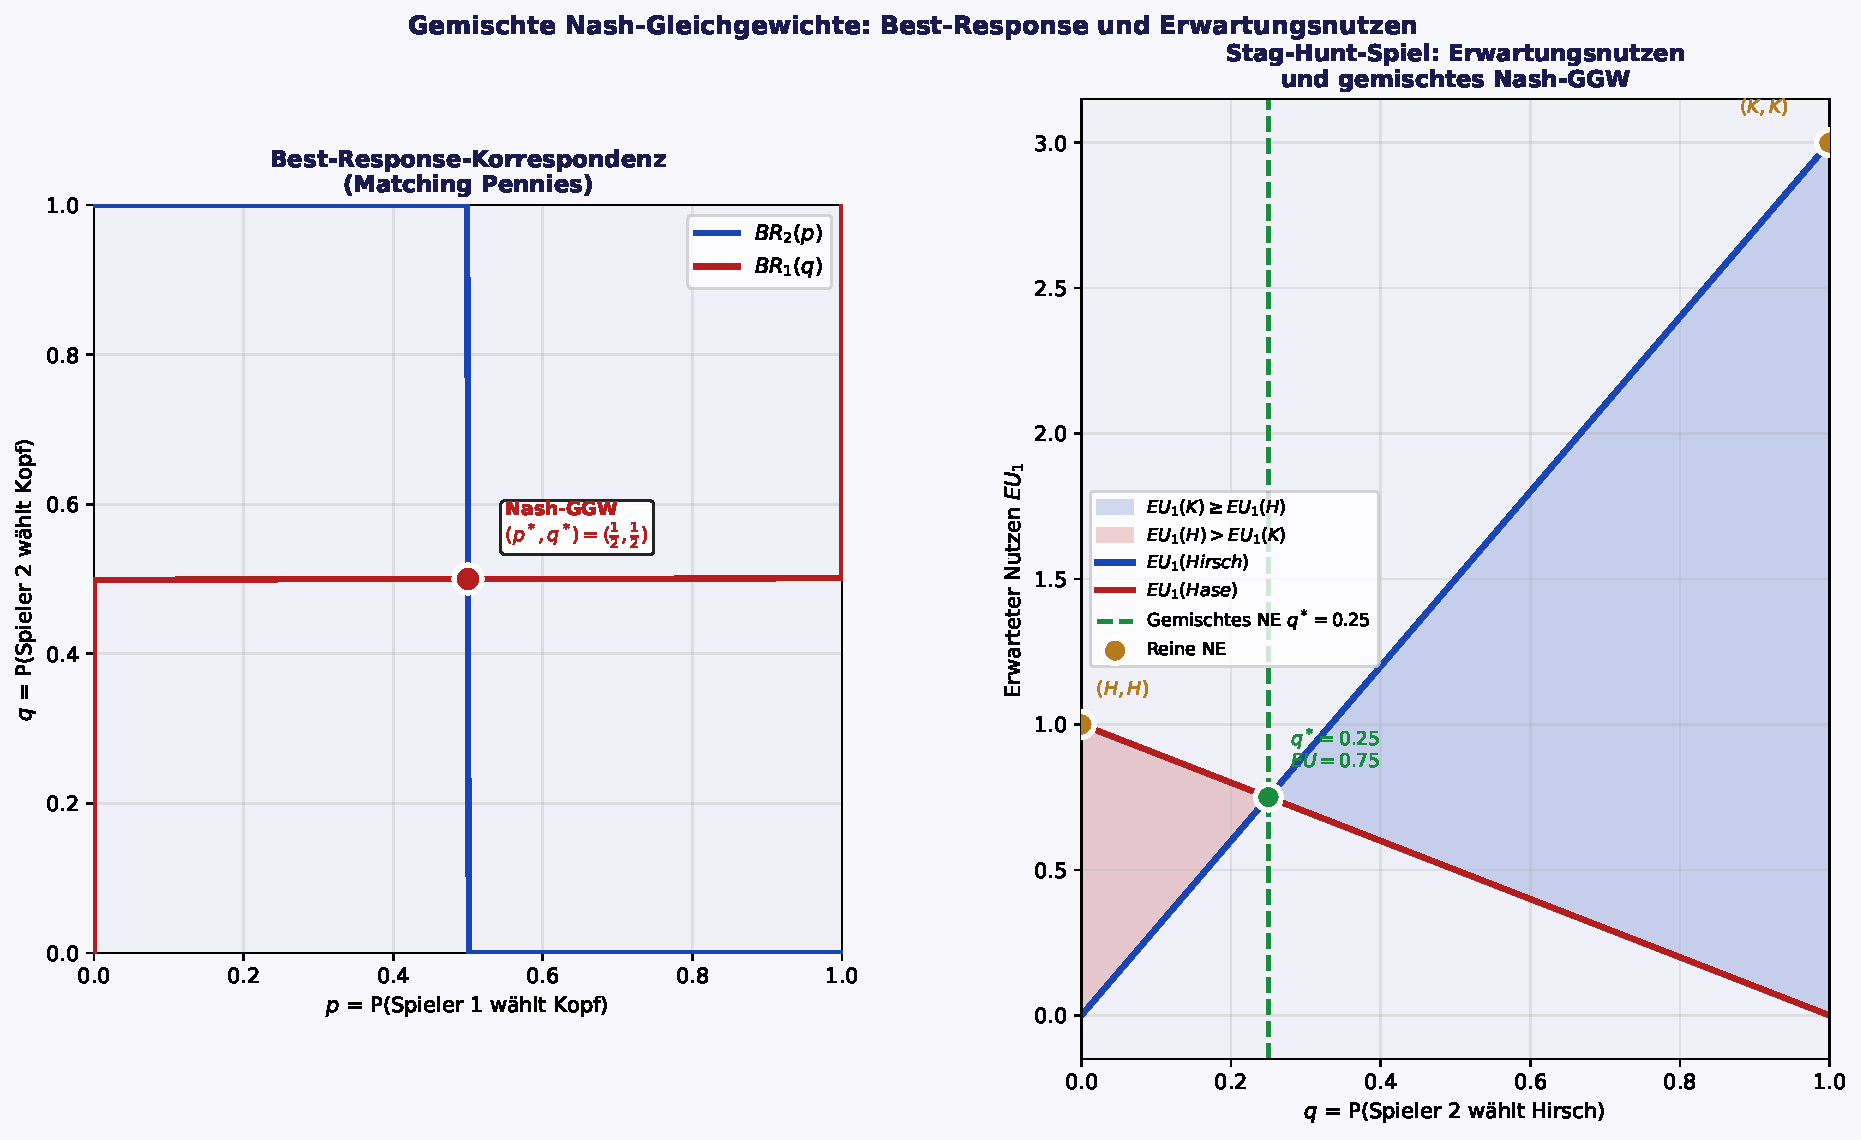
\includegraphics[width=0.95\textwidth]{plot4_gemischte_ne.pdf}
\caption{Links: Best-Response-Korrespondenz des Matching-Pennies-Spiels;
$BR_1(q)$ (rot) und $BR_2(p)$ (blau) schneiden sich im eindeutigen gemischten
Nash-GGW $(p^*, q^*) = (1/2, 1/2)$.
Rechts: Stag-Hunt-Spiel -- Erwartungsnutzen als Funktion von $q$; zwei reine
Nash-GGW (Hirsch,Hirsch) und (Hase,Hase) und ein gemischtes Nash-GGW bei
$q^* = 1/3$, das durch den Kreuzungspunkt der Erwartungsnutzenfunktionen definiert wird.}
\label{fig:gemischte_ne}
\end{figure}

%%%%%%%%%%%%%%%%%%%%%%%%%%%%%%%%%%%
\section{Evolutionäre Spieltheorie und Replikatordynamik}
%%%%%%%%%%%%%%%%%%%%%%%%%%%%%%%%%%%

\begin{definition}[Evolutionär Stabile Strategie]
Eine reine Strategie $p^* \in \Delta(S)$ ist \emph{evolutionär stabil} (ESS),
wenn f\"ur alle $q \neq p^*$ ein $\bar{\varepsilon} > 0$ existiert, sodass
f\"ur alle $\varepsilon \in (0, \bar{\varepsilon})$ gilt:
\[
u(p^*, \varepsilon q + (1-\varepsilon)p^*) > u(q, \varepsilon q + (1-\varepsilon)p^*).
\]
\end{definition}

\begin{satz}[Replikatordynamik-Konvergenz zum ESS]
\label{satz:replikator}
Im Hawk-Dove-Spiel mit Ressourcenwert $V > 0$ und Kampfkosten $C > V$
konvergiert die Replikatordynamik
\[
\dot{p} = p\,(1-p)\left[\bar{f}_H(p) - \bar{f}_D(p)\right]
\]
f\"ur alle Startwerte $p_0 \in (0,1)$ zum evolutionär stabilen Gleichgewicht
\[
p^* = \frac{V}{C}.
\]
\end{satz}

\begin{proof}
\textbf{Schritt 1: Fitnessfunktionen.}
Bei Hawk-Anteil $p$ sind die erwarteten Fitnesswerte:
\begin{align*}
\bar{f}_H(p) &= p \cdot \frac{V-C}{2} + (1-p) \cdot V = V - p\frac{V+C}{2}, \\
\bar{f}_D(p) &= p \cdot 0 + (1-p) \cdot \frac{V}{2} = \frac{V(1-p)}{2}.
\end{align*}

\textbf{Schritt 2: Gleichgewichtsbedingung.}
$\bar{f}_H(p^*) = \bar{f}_D(p^*)$:
\[
V - p^* \frac{V+C}{2} = \frac{V(1-p^*)}{2}
\;\Rightarrow\; p^* = \frac{V}{C}.
\]

\textbf{Schritt 3: Stabilit\"at.}
Definiere $g(p) = \bar{f}_H(p) - \bar{f}_D(p)$. Dann:
\[
g(p) = V - p\frac{V+C}{2} - \frac{V(1-p)}{2} = \frac{V}{2} - p\frac{C}{2}
= \frac{C}{2}\left(\frac{V}{C} - p\right).
\]
Also: $g(p) > 0$ f\"ur $p < p^*$ (Hawk w\"achst) und $g(p) < 0$ f\"ur $p > p^*$
(Hawk schrumpft). Die Ableitung $\dot{p} = p(1-p)g(p)$ hat bei $p^*$ einen
einfachen Nulldurchgang mit negativer Steigung -- $p^*$ ist asymptotisch stabil.
Im Spielgraphen $G_\Gamma$ entspricht $p^*$ einer stabilen Senke des
deterministischen Flusses.
\end{proof}

\begin{figure}[h!]
\centering
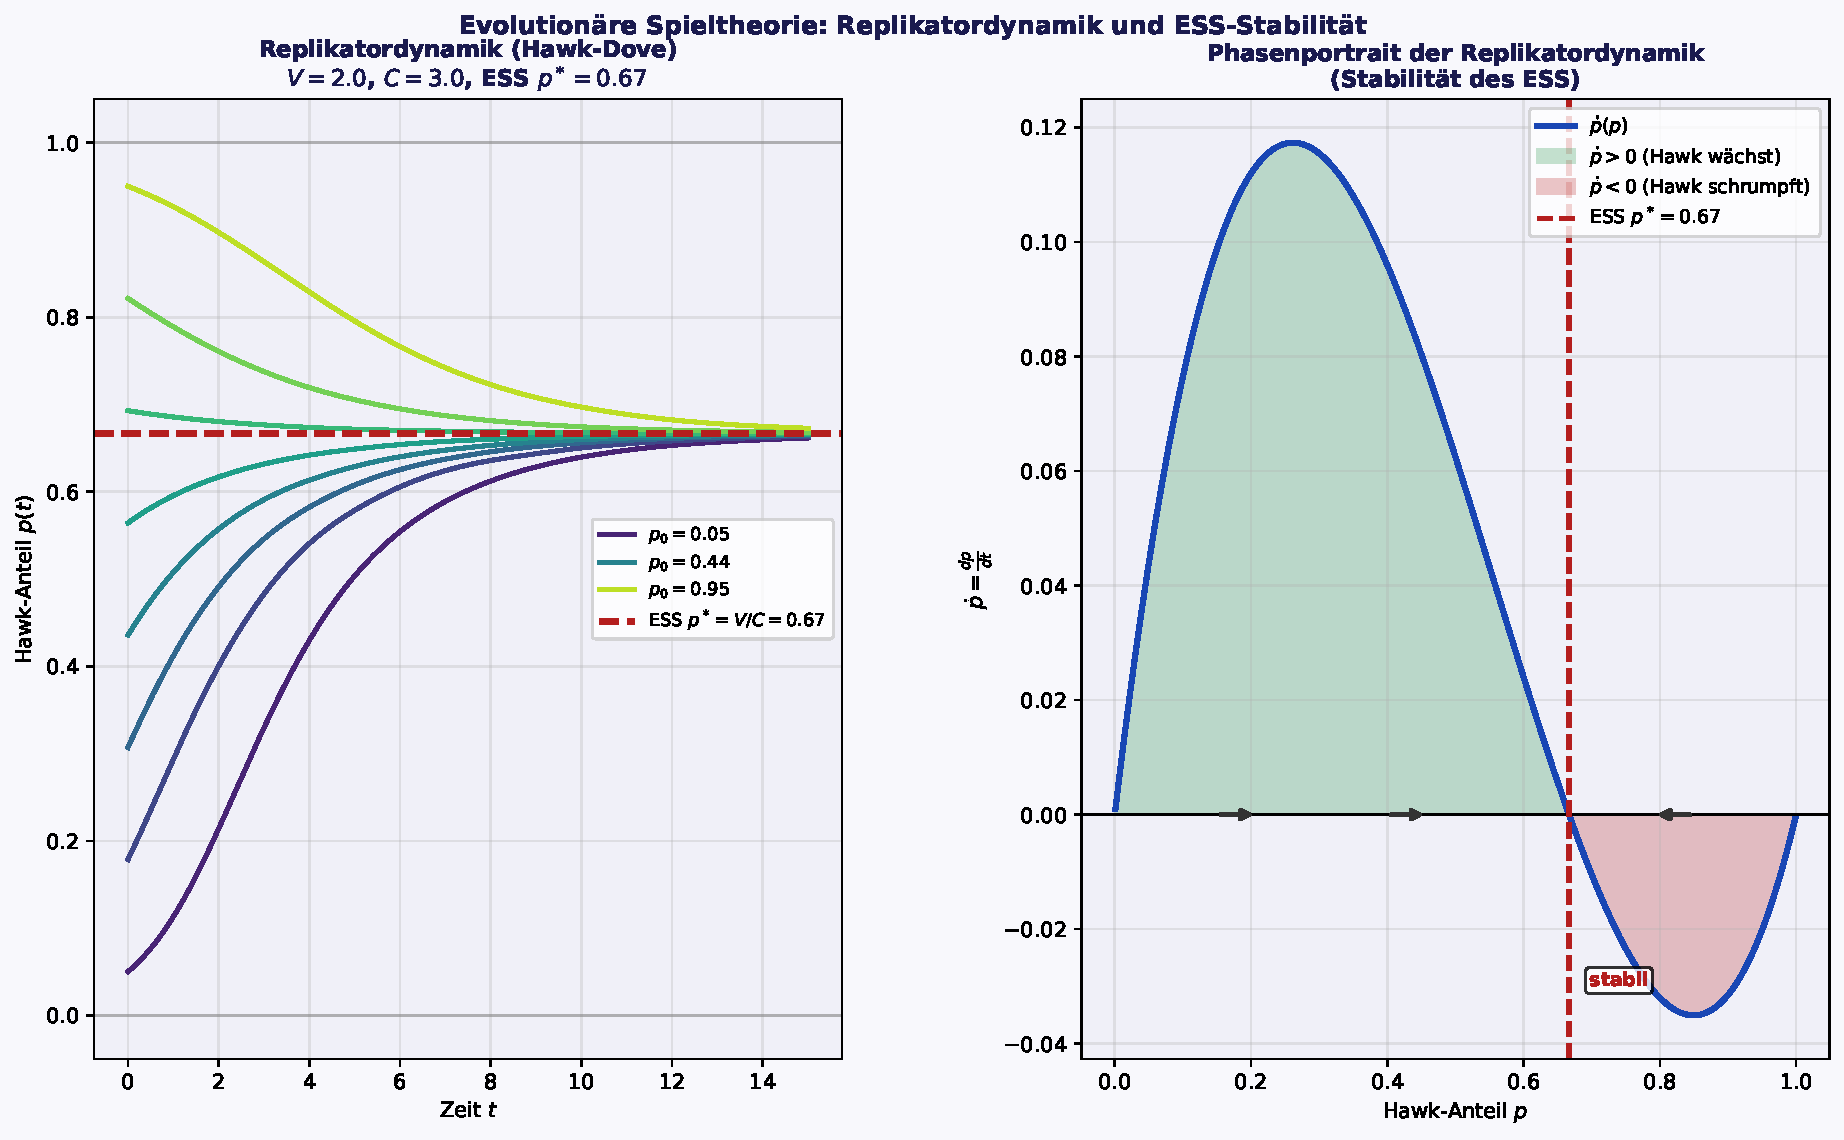
\includegraphics[width=0.95\textwidth]{plot5_replikator.pdf}
\caption{Links: Replikatordynamik-Trajektorien (Hawk-Dove, $V=2$, $C=3$)
f\"ur verschiedene Startwerte; alle konvergieren gegen ESS $p^* = V/C = 0.67$.
Rechts: Phasenportrait $\dot{p}(p)$; gr\"une/rote Fl\"achen kennzeichnen
wachsenden/schrumpfenden Hawk-Anteil; Pfeile zeigen Flussrichtung.}
\label{fig:replikator}
\end{figure}

%%%%%%%%%%%%%%%%%%%%%%%%%%%%%%%%%%%
\section{Koalitionale Spieltheorie und Shapley-Wert}
%%%%%%%%%%%%%%%%%%%%%%%%%%%%%%%%%%%

\begin{definition}[Koalitionsspiel mit \"ubertragbarem Nutzen]
Ein \emph{koalitionales Spiel} ist ein Paar $(N, v)$ mit
$N = \{1,\ldots,k\}$ (Spieler) und
$v: 2^N \to \mathbb{R}$ (charakteristische Funktion) mit $v(\emptyset) = 0$.
\end{definition}

\begin{definition}[Shapley-Wert]
Der \emph{Shapley-Wert} von Spieler $i$ ist:
\[
\phi_i(v) = \sum_{S \subseteq N \setminus \{i\}}
\frac{|S|!\,(|N|-|S|-1)!}{|N|!}
\left[v(S \cup \{i\}) - v(S)\right].
\]
\end{definition}

\begin{satz}[Axiomatische Charakterisierung des Shapley-Werts]
\label{satz:shapley_axio}
Der Shapley-Wert ist die eindeutige Verteilungsregel, die gleichzeitig
folgende vier Axiome erf\"ullt:
\begin{itemize}
    \item \textbf{Effizienz:} $\sum_{i \in N} \phi_i = v(N)$,
    \item \textbf{Symmetrie:} Austauschbare Spieler erhalten gleiche Auszahlungen,
    \item \textbf{Nullspieler:} $\phi_i = 0$ falls $v(S \cup \{i\}) = v(S)$
          f\"ur alle $S$,
    \item \textbf{Additivit\"at:} $\phi_i(v+w) = \phi_i(v) + \phi_i(w)$.
\end{itemize}
\end{satz}

\begin{proof}
\textbf{Existenz:} Die Shapley-Wert-Formel erf\"ullt alle vier Axiome per
Konstruktion. Effizienz folgt aus $\sum_{i} \phi_i = v(N)$ (vollst\"andige
Aufteilung der gro{\ss}en Koalition). Symmetrie und Nullspieler folgen direkt
aus der Formel. Additivit\"at: $\phi_i(v+w) = \sum_S w_S [(v+w)(S\cup\{i\})
- (v+w)(S)] = \phi_i(v) + \phi_i(w)$.

\textbf{Eindeutigkeit:} Jede Valuation $v$ l\"asst sich als Linearkombination
von Einheitsspielen $u_T$ (mit $u_T(S) = 1$ gdw.\ $T \subseteq S$,
sonst $0$) schreiben: $v = \sum_T c_T u_T$.
F\"ur Einheitsspiele ist der einzige Wert, der alle vier Axiome erf\"ullt,
durch $\phi_i(u_T) = 1/|T|$ f\"ur $i \in T$ (Symmetrie) und $0$ sonst
(Nullspieler) bestimmt. Durch Additivit\"at folgt die Eindeutigkeit f\"ur
allgemeine $v$~\cite{shapley1953}.
\end{proof}

\begin{korollar}[Shapley-Wert als fairer Absorptionspunkt]
Im Koalitionsgraphen $G_\mathcal{K}$ (Satz~\ref{satz:nash_subgraph} angewendet
auf koalitionale Spiele) entspricht die Shapley-Wert-Allokation $(\phi_i)_{i \in N}$
dem eindeutigen fairen Absorptionspunkt: Sie ist der einzige
Auszahlungsvektor, den kein Spieler durch Wechsel in eine andere Koalition
verbessern kann, ohne die Fairness-Axiome zu verletzen.
\end{korollar}

\begin{figure}[h!]
\centering
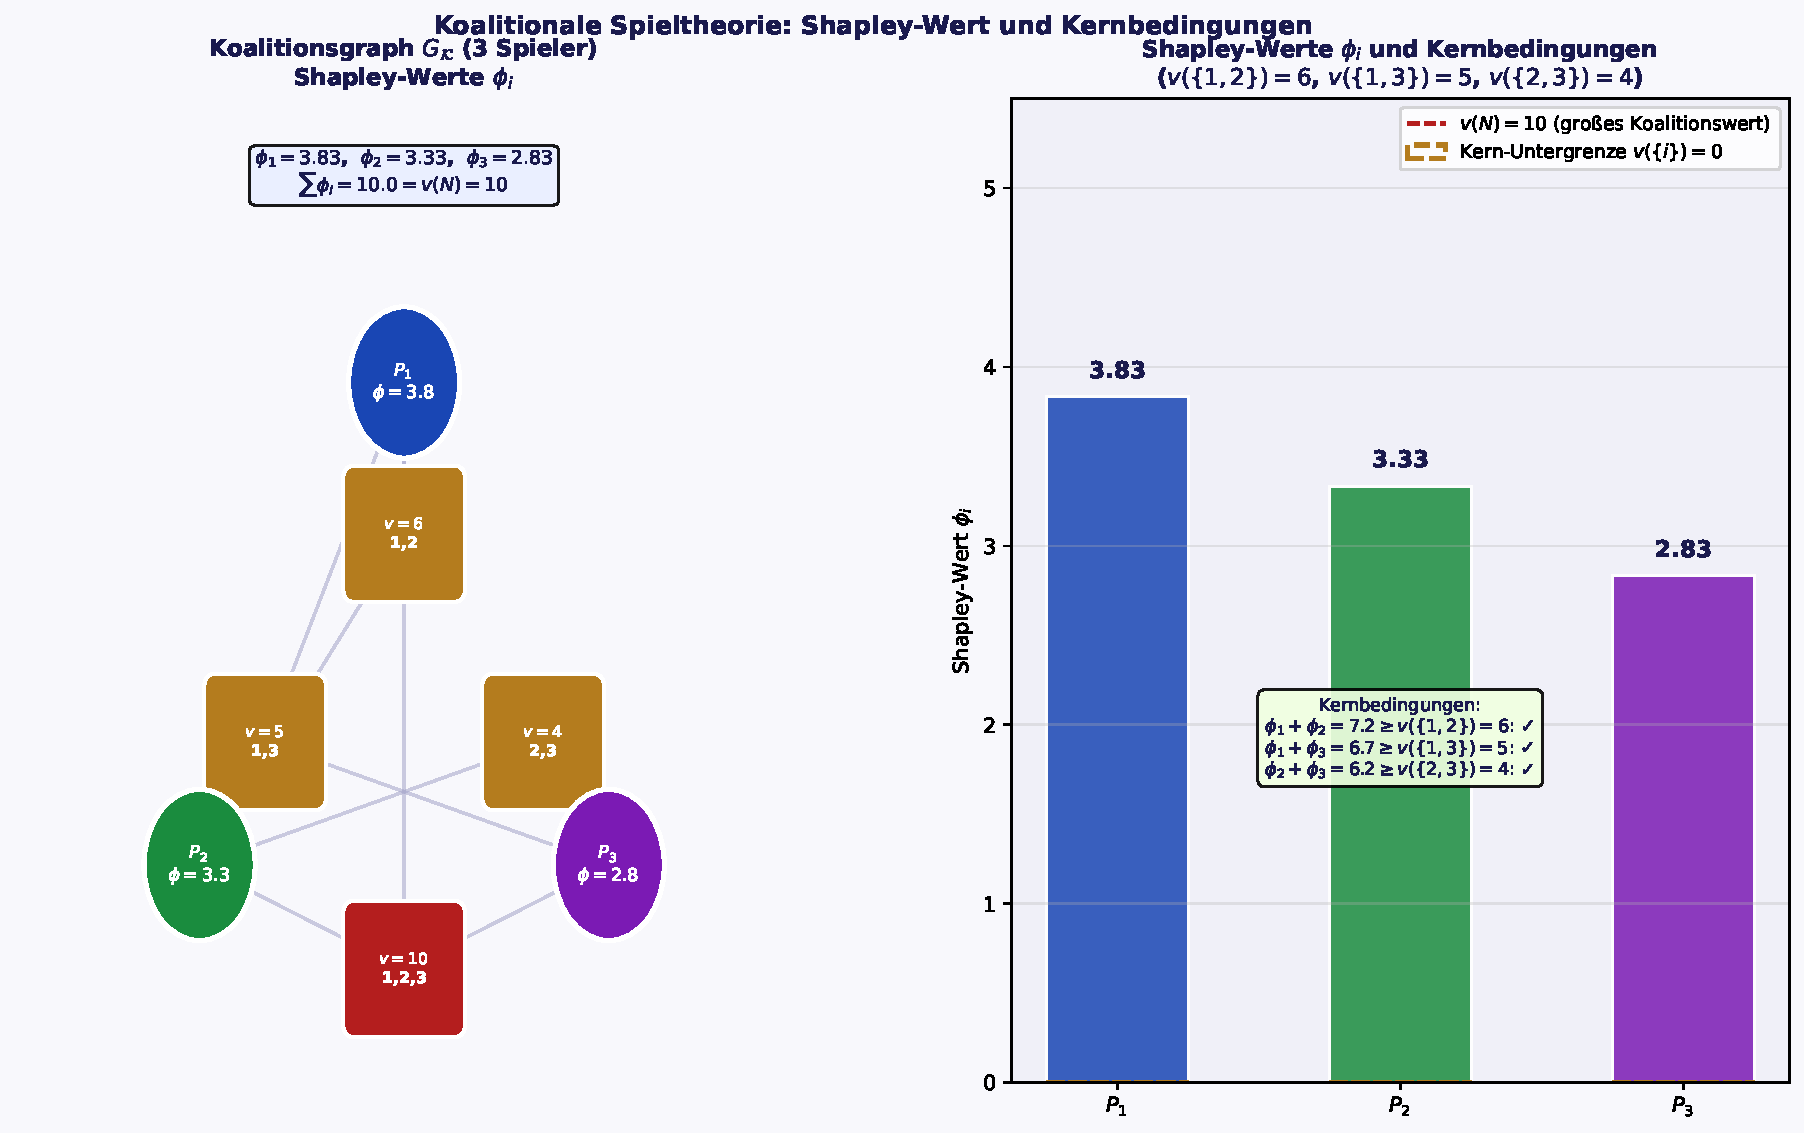
\includegraphics[width=0.95\textwidth]{plot6_shapley.pdf}
\caption{Links: Koalitionsgraph $G_\mathcal{K}$ f\"ur 3 Spieler;
Spieler-Knoten (blau/gr\"un/lila) mit Shapley-Werten $\phi_i$,
Koalitionsknoten mit charakteristischen Funktionswerten $v(S)$.
Rechts: Balkendiagramm der Shapley-Werte; Kernbedingungen
$\phi_i + \phi_j \geq v(\{i,j\})$ sind als Stabilit\"atspr\"ufung annotiert.}
\label{fig:shapley}
\end{figure}

%%%%%%%%%%%%%%%%%%%%%%%%%%%%%%%%%%%
\section{Zusammenfassung}
%%%%%%%%%%%%%%%%%%%%%%%%%%%%%%%%%%%

Diese Arbeit hat eine vollst\"andige graphentheoretische Behandlung der
Spieltheorie entwickelt. Die zentralen Ergebnisse:

\begin{itemize}
    \item \textbf{Satz~\ref{satz:nash_subgraph}} (Nash als Senke):
          Nash-Gleichgewichte sind Absorptionsknoten im Spielgraphen.
    \item \textbf{Korollar~\ref{kor:linsuche}} (Lineare Suche):
          Alle Nash-GGW in $O(|S|^2 \cdot |N|)$.
    \item \textbf{Satz~\ref{satz:strat_iso}} (Strategische Isomorphie):
          \"Aquivalenz via Subgraph-Algorithmus in $O(n^3)$.
    \item \textbf{Satz~\ref{satz:teilspiel}} (Teilspiel):
          Teilspiele als Subgraphen.
    \item \textbf{Satz~\ref{satz:walras_nash}} (Walras-Nash):
          Walrasianisches GGW ist Nash-GGW.
    \item \textbf{Satz~\ref{satz:knotengleichgewicht}} (Knotengleichgewicht):
          \"Okonomisches Kirchhoff-Gesetz an Marktknoten.
    \item \textbf{Satz~\ref{satz:nash_existenz}} (Existenz):
          Kakutani-Fixpunktsatz garantiert gemischtes Nash-GGW.
    \item \textbf{Satz~\ref{satz:replikator}} (Replikator):
          ESS als stabiler Attraktor der Replikatordynamik.
    \item \textbf{Satz~\ref{satz:shapley_axio}} (Shapley):
          Axiomatische Charakterisierung und Eindeutigkeit.
\end{itemize}

%%%%%%%%%%%%%%%%%%%%%%%%%%%%%%%%%%%
\section{Ausblick}
%%%%%%%%%%%%%%%%%%%%%%%%%%%%%%%%%%%

\subsection{Polynomielle Berechnung von Correlated-Equilibria}

Das Nash-Gleichgewicht ist nicht das einzige Gleichgewichtskonzept.
\emph{Korrelierte Gleichgewichte} (Aumann 1974~\cite{aumann1974}) verallgemeinern
Nash: Ein gemeinsames Zufallssignal koordiniert die Spieler.
Im Spielgraphen $G_\Gamma$ entspricht ein korreliertes Gleichgewicht einer
Wahrscheinlichkeitsverteilung $\mu$ \"uber $S$, sodass f\"ur alle $i$ und $s_i$:
\[
\sum_{s_{-i}} \mu(s_i, s_{-i}) [u_i(s_i', s_{-i}) - u_i(s_i, s_{-i})] \leq 0.
\]
Dies ist ein lineares Programm in $|S|$ Variablen.
Forschungsfrage: Kann der Subgraph-Algorithmus~\cite{epp2026subgraph} die
LP-Struktur der korrelierten Gleichgewichte beschleunigen?
Konkret: Die Signaturen des Spielgraphen liefern eine kompakte Repr\"asentation
der LP-Koeffizientenmatrix, was die Pivotierung im Simplex-Algorithmus
auf $O(n^2)$ pro Schritt statt $O(n^3)$ reduzieren k\"onnte.

\subsection{Makro\"okonomische Gleichgewichtsmodelle als Spielgraphen}

Das Systemzustandsmodell~\cite{epp2026sysstate} beschreibt \"Uberg\"ange zwischen
wirtschaftlichen Zust\"anden (Expansion, Rezession, Krise) als Markov-Kette.
Dies ist strukturell isomorph zum Spielgraphen $G_{\mathrm{sys}}$:
Zust\"ande sind Knoten, \"Ubergangswahrscheinlichkeiten sind Kantengewichte,
und der Gleichgewichtszustand ist der Absorptionsknoten.

Der Subgraph-Algorithmus erm\"oglicht es, wiederkehrende makro\"okonomische
Muster in historischen Zeitreihen als Subgraphen zu identifizieren:
Ist die aktuelle Konjunkturphase ein Teilgraph der Gro{\ss}en Depression
(1929--1933)? Ist sie ein Teilgraph der Dot-com-Blase (2000--2003)?
Jede historische Episode wird als Signatur-Array kodiert;
der $O(n^3)$-Algorithmus entscheidet Strukturgleichheit in Echtzeit.

\subsection{Spieltheorie in heterogenen Mobilfunknetzen}

Das heterogene Netzwerkmodell~\cite{epp2026hetnet} beschreibt Ressourcenallokation
in Mobilfunknetzen als POMDP. Netzwerkknoten (Basisstationen, mobile Ger\"ate)
spielen ein Spiel um Bandbreite, Energie und Latenz.
Das Nash-Gleichgewicht dieses Netzwerkspiels ist der optimale Betriebspunkt.

Formale Verbindung: Das Netzwerkspiel $\Gamma_{\mathrm{Net}}$ hat als Spielgraphen
$G_{\Gamma_{\mathrm{Net}}} \subseteq G_\Gamma$, wobei $G_\Gamma$ das vollst\"andige
Strategieprofil-Graph ist. Der Subgraph-Algorithmus~\cite{epp2026subgraph}
identifiziert optimale Teilgraphen (optimale Konfigurationen) in $O(n^3)$.
Verbindung zu RL: Der Reinforcement-Learning-Agent aus~\cite{epp2026hetnet}
konvergiert zum Nash-GGW des Netzwerkspiels; der Spielgraph liefert die
formale Konvergenzgarantie.

\subsection{Marktdesign und Mechanismus-Design via Graphentheorie}

Mechanismus-Design (umgekehrte Spieltheorie) fragt: Wie gestaltet man ein
Spielregelwerk, sodass das resultierende Nash-GGW sozial optimal ist?
Im Spielgraphen-Framework entspricht dies der Frage: Wie ver\"andert man
$E_{\mathrm{BR}}$, sodass der gew\"unschte Knoten $s^{\mathrm{opt}}$ zur einzigen
Senke wird?

Formale Verbindung zum lokalen \"okonomischen Modell~\cite{epp2026leco}:
Das \texttt{leco}-Modell beschreibt lokale Marktgleichgewichte als Fixpunkte
lokaler Optimierungsprobleme. Durch Anpassung der Spielregeln (Steuern,
Subventionen, Regulierungen) als Kantengewichte in $G_\Gamma$ kann das
gew\"unschte Gleichgewicht gezielt konstruiert werden.
Der Subgraph-Algorithmus pr\"uft in $O(n^3)$, ob die gew\"unschte
Senkenstruktur im modifizierten Spielgraphen realisiert wird.

\subsection{Rentenmarkt-Spiele und das Abh\"angigkeitsmodell}

Das Abh\"angigkeitsmodell~\cite{epp2026depension} formalisiert intertemporale
Umverteilungsentscheidungen im Rentenmarkt.
In spieltheoretischer Interpretation: Aktive Einzahler und Rentenempf\"anger
spielen ein Spiel um Einzahlungss\"atze, Rentenh\"ohe und Nachhaltigkeitsziel.

Das Nash-Gleichgewicht des Rentenspiels:
$(\text{Einzahlungssatz}^*, \text{Rentenniveau}^*)$ minimiert
soziale Unzufriedenheit \"uber alle Generationen, wenn kein Akteur durch
einseitige \"Anderung profitiert (intergenerationales Nash-GGW).
Der Spielgraph $G_{\mathrm{Rente}}$ verbindet Generationen als Knoten;
Kantengewichte kodieren \"Ubertragungsraten.
Subgraph-Analyse: Welche historischen Rentenmodelle (Bismarck 1889,
Bismarck-Reformen 1950er, Riester 2002) sind subgraphisomorph?

\subsection{Klimakooperationsspiele}

Klimaverhandlungen (Paris-Abkommen, Kyoto-Protokoll) sind Kooperationsspiele
unter Externali\"aten. Jede Nation $i$ hat eine Emissionsstrategiemenge
$S_i = [0, e_i^{\max}]$ und Nutzenfunktion
$u_i(e) = B_i(e_i) - D_i(\sum_j e_j)$
(privater Nutzen aus Emissionen minus globaler Klimaschaden).

Das Nash-GGW des Klimaspiels $e^* = (e_i^*)$ erf\"ullt
$B_i'(e_i^*) = 0$ (da $D_i$ die Externalit\"at vernachl\"assigt bei
nichtkooperativem Verhalten): \"Uberm\"a{\ss}ige Emissionen.
Das soziale Optimum $e^{\mathrm{opt}}$ mit
$B_i'(e_i^{\mathrm{opt}}) = \sum_j D_j'(\sum e_j)$ (Pigou-Steuer)
ist ein anderer Knoten im Spielgraphen.
Verbindung zur atmosph\"arischen Systemtheorie~\cite{epp2026klima}:
Das Klimaspiel ist in den atmosph\"arischen Systemzustandsgraphen eingebettet.

\subsection{Spieltheoretische Analyse von Epidemien}

Epidemien (SIR-Modell~\cite{epp2026r0}) k\"onnen spieltheoretisch interpretiert
werden: Jedes Individuum spielt ein Spiel zwischen Impfung ($I$) und
Nichtimpfung ($NI$). Das Nash-GGW ist das Gleichgewicht zwischen
privaten Impfkosten und H\"{e}rdenimmunit\"at.

Im Spielgraphen: $(I, \ldots, I)$ ist Nash-GGW nur wenn $R_0 > 1$
und Impfung dominante Strategie ist; bei $R_0 < 1$ ist $(NI, \ldots, NI)$
Nash-GGW (Trittbrettfahrerproblem).
Der Subgraph-Algorithmus identifiziert \"ahnliche Gleichgewichtsmuster
in verschiedenen Epidemien (COVID-19, Ebola~\cite{epp2026ebola},
Hantavirus~\cite{epp2026hantavirus}) durch Signatur-Vergleich der
epidemiologischen Spielgraphen.

\subsection{Post-Quanten-Kryptographie als Spieltheorie}

Das Kryptosystem-Design ist ein Spiel zwischen Angreifer und Verteidiger.
In der gitterbasierten Kryptographie~\cite{epp2026lattice} spielt der
Angreifer das SVP-Spiel (Shortest Vector Problem); der Verteidiger
parametrisiert das Gitter.
Das Nash-GGW: Angreifer spielt h\"arten SVP-Algorithmus, Verteidiger w\"ahlt
optimale Gitterparameter.
Formal: Das Kryptospiel $\Gamma_{\mathrm{Krypto}}$ hat als Spielgraphen
$G_{\Gamma_{\mathrm{Krypto}}}$; das Sicherheitsniveau entspricht dem
Auszahlungsunterschied zwischen Nash-GGW und sozialem Optimum des Spiels.

\subsection{Quantenspiele und Quantengleichgewichte}

Quantencomputer~\cite{epp2026quantum} erm\"oglichen \emph{Quantenspiele}:
Spieler k\"onnen verschr\"ankte Quantenstrategien $|\psi\rangle$ spielen statt
klassischer gemischter Strategien.
Das bekannteste Ergebnis (Eisert, Wilkens, Lewenstein 1999): Im
Quantengefangenendilemma kann durch Verschr\"ankung das Pareto-optimale
$(C,C)$ als Nash-GGW realisiert werden, das im klassischen Spiel nicht stabil ist.

Im Spielgraph-Framework: Quantenstrategien erweitern den Strategieraum
von $\Delta(S)$ auf die unit\"are Gruppe $U(2^k)$ (f\"ur $k$ Qubits).
Der Spielgraph $G_{\Gamma_Q}$ hat exponentiell mehr Knoten;
der Subgraph-Algorithmus~\cite{epp2026subgraph} auf dem quantenerweiterten
Spielgraphen erm\"oglicht die Identifikation von Quantengleichgewichten als
Subgraphen klassischer Equilibria.

\subsection{Netzwerkspiele und soziale Netzwerke}

In sozialen Netzwerken spielen Agenten Spiele auf Graphen (Braess-Paradoxon,
Routing-Spiele~\cite{roughgarden2005}). Die Netzwerktopologie beeinflusst
direkt die Nash-Gleichgewichte.
Verbindung zum Subgraph-Algorithmus: Zwei soziale Netzwerke mit subgraphisomorphen
Spielgraphen haben strukturell identische Nash-Gleichgewichte.
Dies erm\"oglicht die \"Ubertragung von Erkenntnissen zwischen verschiedenen
sozialen Kontexten (z.\,B.\ Impfentscheidungen in verschiedenen
Bev\"olkerungsnetzwerken).

\subsection{Formale Verifikation von Marktmechanismen}

Spieltheoretische Mechanismen (Auktionen, M\"arkte, Wahlsysteme) k\"onnen
durch den Subgraph-Algorithmus formal verifiziert werden:
Ist der gew\"unschte Mechanismus (Vickrey-Auktion~\cite{vickrey1961}) subgraphisomorph
zum implementierten Algorithmus?
Das ist ein Korrektheitsproblem: Die Signaturen des theoretischen Modells
und der tats\"achlichen Implementierung werden verglichen.
\"Ubereinstimmung (LCS $= n$) garantiert strategische \"Aquivalenz;
Nichtübereinstimmung zeigt Design-Fehler auf.

%%%%%%%%%%%%%%%%%%%%%%%%%%%%%%%%%%%
\begin{thebibliography}{99}
%%%%%%%%%%%%%%%%%%%%%%%%%%%%%%%%%%%

\bibitem{vonneumann1944}
Von Neumann, J., \& Morgenstern, O. (1944).
\textit{Theory of Games and Economic Behavior}.
Princeton University Press.

\bibitem{nash1950}
Nash, J. F. (1950).
Equilibrium points in $n$-person games.
\textit{Proceedings of the National Academy of Sciences}, 36(1), 48--49.

\bibitem{nash1951}
Nash, J. F. (1951).
Non-cooperative games.
\textit{Annals of Mathematics}, 54(2), 286--295.

\bibitem{nobel1994}
Royal Swedish Academy of Sciences (1994).
\textit{The Nobel Prize in Economic Sciences}.
Prize announcement for Nash, Harsanyi, Selten.

\bibitem{kakutani1941}
Kakutani, S. (1941).
A generalization of Brouwer's fixed point theorem.
\textit{Duke Mathematical Journal}, 8(3), 457--459.

\bibitem{shapley1953}
Shapley, L. S. (1953).
A value for $n$-person games.
\textit{Annals of Mathematics Studies}, 28, 307--317.

\bibitem{maynardsmith1973}
Maynard Smith, J., \& Price, G. R. (1973).
The logic of animal conflict.
\textit{Nature}, 246(5427), 15--18.

\bibitem{aumann1974}
Aumann, R. J. (1974).
Subjectivity and correlation in randomized strategies.
\textit{Journal of Mathematical Economics}, 1(1), 67--96.

\bibitem{monderer1996}
Monderer, D., \& Shapley, L. S. (1996).
Potential games.
\textit{Games and Economic Behavior}, 14(1), 124--143.

\bibitem{roughgarden2005}
Roughgarden, T. (2005).
\textit{Selfish Routing and the Price of Anarchy}.
MIT Press.

\bibitem{fudenberg1991}
Fudenberg, D., \& Tirole, J. (1991).
\textit{Game Theory}.
MIT Press.

\bibitem{konig1936}
K\"onig, D. (1936).
\textit{Theorie der endlichen und unendlichen Graphen}.
Leipzig: Akademische Verlagsgesellschaft.

\bibitem{vickrey1961}
Vickrey, W. (1961).
Counterspeculation, auctions, and competitive sealed tenders.
\textit{Journal of Finance}, 16(1), 8--37.

\bibitem{epp2026subgraph}
Epp, S. (2026).
Der Subgraph Algorithmus -- L\"osung des Subgraph-Isomorphismus in $O(n^3)$.
Universit\"at Bielefeld.
\url{https://gitlab.com/epp-group/subgraph}

\bibitem{epp2026sysstate}
Epp, S. (2026).
Systemzust\"ande und dynamische Gleichgewichtsmodelle.
Google Drive (epp-group).

\bibitem{epp2026leco}
Epp, S. (2026).
Lokales \"okonomisches Modell (leco) -- Marktstrukturen und Gleichgewichte.
Google Drive (epp-group).

\bibitem{epp2026depension}
Epp, S. (2026).
Abh\"angigkeitsmodell (depension) -- Intertemporale Rentenmarktoptimierung.
Google Drive (epp-group).

\bibitem{epp2026knoten}
Epp, S. (2026).
Die Knotengleichung als universelles Naturgesetz.
Google Drive (epp-group).

\bibitem{epp2026hetnet}
Epp, S. (2026).
Lernbasiertes autonomes Netzwerkmanagement in heterogenen Mobilfunknetzen.
Google Drive (epp-group).

\bibitem{epp2026klima}
Epp, S. (2026).
Atmosph\"arische Systemtheorie -- Graphentheoretische Formalisierung.
Google Drive (epp-group).

\bibitem{epp2026lattice}
Epp, S. (2026).
Gitterbasierte Kryptographie und Quanten-Fehlerkorrektur.
Google Drive (epp-group).

\bibitem{epp2026quantum}
Epp, S. (2026).
Quantenzust\"ande, Verschr\"ankung und Koh\"arenz.
Universit\"at Bielefeld.

\bibitem{epp2026r0}
Epp, S. (2026).
Basisreproduktionszahl $R_0$ -- Formale Klassifikation epidemiologischer
Ausbreitungsklassen.
Google Drive (epp-group).

\bibitem{epp2026ebola}
Epp, S. (2026).
Ebola-Ausbreitungsmodell via Subgraph-Algorithmen.
Google Drive (epp-group).

\bibitem{epp2026hantavirus}
Epp, S. (2026).
Graphentheoretische Modellierung und Analyse des Hantavirus.
Google Drive (epp-group).

\end{thebibliography}

\end{document}
